\chapter{Literature Study}

The literature study introduces the reader to a few fundamental concepts, and similar implementations to give context to the project. It also briefly evaluates cost effectiveness.\\

Infrared light extends from the nominal `red edge' of the visible spectrum at 700 nanometers (430 THz) to 1 mm (300 GHz) \cite{ir_wiki}. Due to the silicon response, the image sensor in consumer cameras can capture infra-red light up to 1000 nanometers \cite{ir_wiki} as in Figure \ref{fig:ir_spectrum} (excluding ultraviolet light). Also, there is a certain phenomenon which occurs within this region. Chlorophyll becomes transparent, and allows each vegetation cell to act as an elementary corner reflector. This accounts for a rapid change in reflectance, depending on the health of the plant, and is utilized in vegetation indices, such as the NDVI \cite{red_edge}.

\begin{figure}[H]
\centering
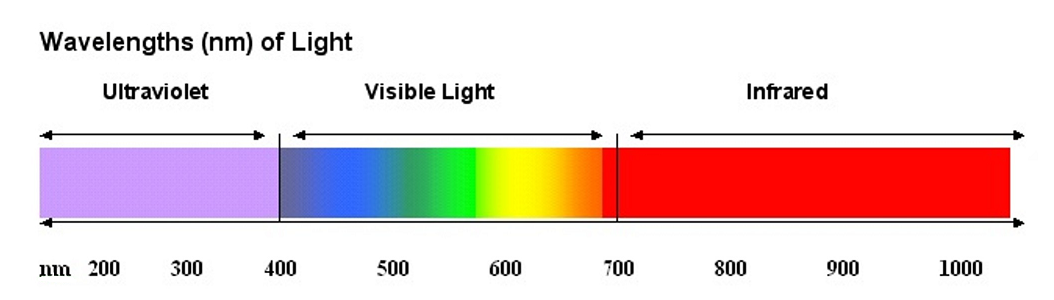
\includegraphics[scale=0.35]{images/ir_spectrum.png}
\caption{Wavelengths of light \cite{ir_spectrum}}
\label{fig:ir_spectrum}
\end{figure}


The normalized difference vegetation index (NDVI), is a simple graphical indicator that can be used to analyze remote sensing measurements, typically from a space platform\footnote{Aerial footage will always be higher resolution, with each pixel capturing under a few $cm^2$ as opposed to under a few $m^2$, and is useful for more in-depth analysis}, and assess whether the target being observed contains live green vegetation or not\cite{ndvi_wiki} as in Figure \ref{fig:ndvi_british}. The higher the values are, the more photosynthetically active the plants are, and in the following two pictures, the colour map ranges from black ($-1.0$) to dark green ($1.0$).

\begin{figure}[H]
\begin{subfigure}{0.5\textwidth}
\centering
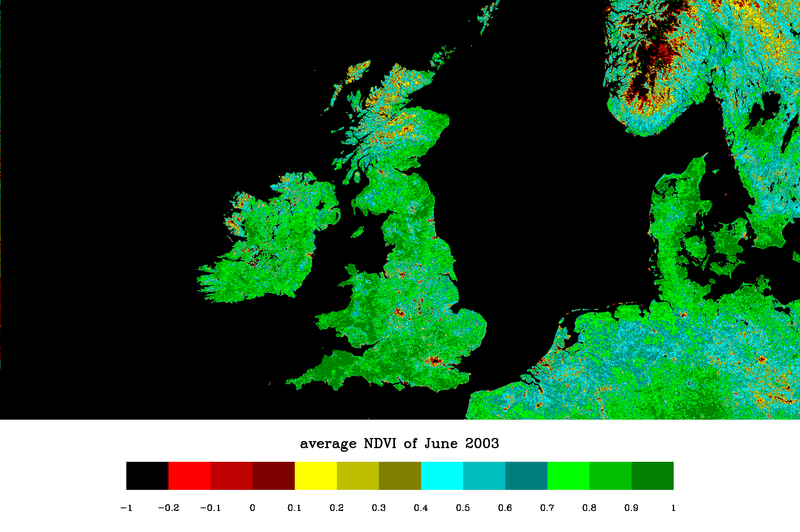
\includegraphics[scale=0.25]{images/NDVI_062003.png}
\caption{Summer in June 2003}
\end{subfigure}
\begin{subfigure}{0.5\textwidth}
\centering
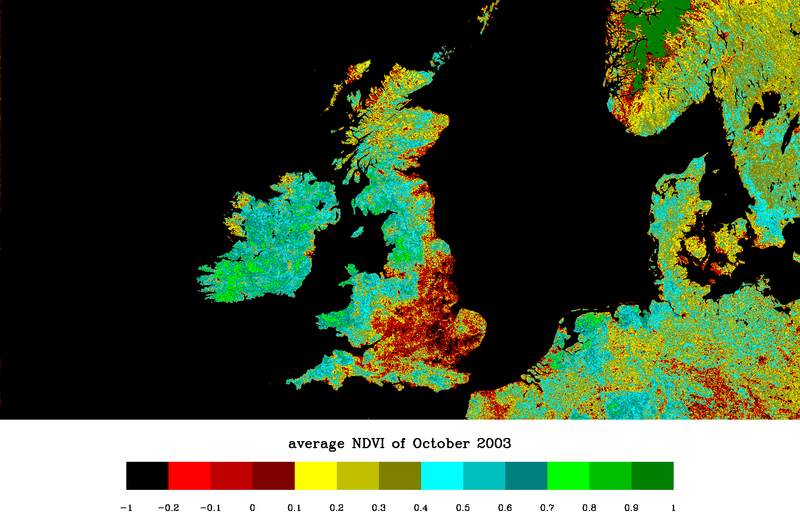
\includegraphics[scale=0.25]{images/NDVI_102003.png}
\caption{Autumn in October 2003}
\end{subfigure}
\caption{Average NDVI over the British Isles \cite{ndvi_wiki}}
\label{fig:ndvi_british}
\end{figure}

The NDVI is calculated using the following formula for each pixel:

\begin{equation}\label{eq:ndvi}
{\displaystyle{\mbox{NDVI}}={\frac {({\mbox{NIR}}-{\mbox{Red}})}{({\mbox{NIR}}+{\mbox{Red}})}}}, \in [-1.0, 1.0]
\end{equation}

where red and NIR stand for the spectral reflectance measurements acquired in the red (visible) and near-infrared regions, respectively.

\begin{figure}[H]
\centering
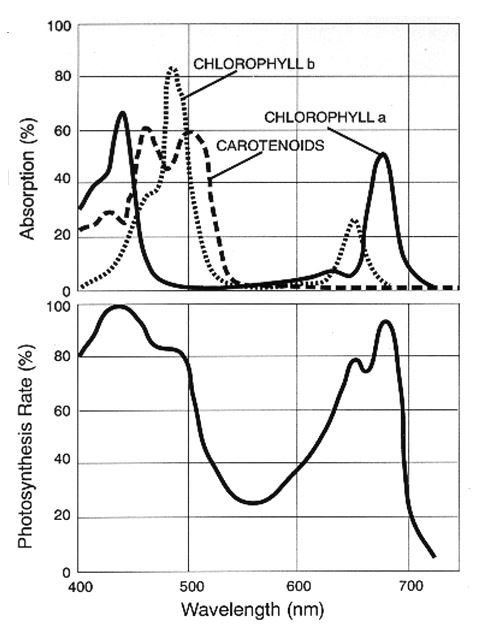
\includegraphics[scale=0.5]{images/chlorophyll.jpg}
\centering
\caption{PAR and absorption spectrum \cite{ndvi_wiki}}
\label{fig:chlorophyll}
\end{figure}

In Figure \ref{fig:chlorophyll}, typical photosynthetic action in the photosynthetically active radiation (PAR) spectral region for live green plants is shown, beside absorption spectra for chlorophyll and carotenoids. Solar radiation is absorbed within this region as a source of energy. \\

Leaf cells re-emit solar radiation in the near-infrared region because the photon energy at wavelengths longer than 700 nm is not large enough to synthesize organic molecules, even though it comprises approximately half of the total incoming solar energy. If it were absorbed, it would only result in damage and overheating of the plant.\\

The NDVI is similar to a mere ratio of infrared light to visible light, except the ratio is not normalised, therefore infinite values can exist.\\

The rationale behind the NDVI is that one can exploit the strong differences in plant reflectance to determine their spatial distribution.\\

The launch of the Sputnik 1 by the Soviet Union in 1957 sparked an interest in meteorological satellites to improve weather forecasting. NDVIs, introduced in the early seventies by the ERTS\footnote{Earth Resources Technology Satellite, or Landsat 1}, remain popular today. \\

Today, for example, one can expect to pay about \$1600 per fortnightly 0.5m resolution photo from the Pléiades satellite constellation\footnote{Very-high-resolution optical earth-imaging satellites via Satellite Imaging Corporation}. There are other sensors with similar pricing, including the WorldView, GeoEye, Kompsat, Quickbird, Gaofen etc.\\Aerobotics, based in Cape Town have quite a cost effective solution, with weekly footage at 500 ZAR per month, however at a low resolution of 10m per pixel. They also charge 80 ZAR per hectare for drone surveys, and 20 ZAR per hectare\footnote{Worldwide average 59.4 Ha\cite{farm_size}, South Africa between 427 - 5799 Ha \cite{farm_size_sa}} if one uploads one's own data. Solutions like these show that it could be beneficial for a farmer to have their very own automated solution.\\

Since the proliferation of UAVs, there has been an increased effort to find more cost effective solutions to commercial applications, not excluding NDVI analysis. Hypothetically, if an inexperienced farmer were to perform NDVIs of their land by themselves, there does exist online platforms to process the imagery. However, imagery may not necessarily be calibrated, and distortions in the lens may create an inaccurate result. Also, the upfront costs of the hardware required may be too much. Typical drones like the Phantom series cost around \$1000-2000. \\Cameras and pricing include:
\begin{itemize}
	\item Parrot Sequoia, 5 cameras, \$3500 \cite{sequoia}
	\item Mapir Survey2, single camera, \$500 \cite{mapir}
	\item AgroCam Pro, dual cameras, \$575 \cite{agrocam}
\end{itemize}

There are other vegetation indices such as the Enhanced vegetation index in Equation \ref{eq:evi},

\begin{equation}\label{eq:evi}
EVI=G\times {\frac  {(NIR-RED)}{(NIR+C1\times RED-C2\times Blue+L)}}
\end{equation}

where NIR, blue and red refer to atmospherically corrected Raleigh and ozone absorption surface reflectances, L refers to background adjustment in canopies that address non-linear, differential NIR, and the coefficients C1, C2 uses the blue band to correct for aerosol influences in the red band. The EVI, as opposed to the more chlorophyll sensitive NDVI, is more responsive to structural canopy variations, including LAI (leaf index area), physiognomy\footnote{External appearance, and growth forms of dominant taxa} and architecture \cite{evi}. Since it has more of a satellite application, this exists outside the scope of the project.\\

Another example is the Normalized difference water index as in Equation \ref{eq:ndwi},

\begin{equation}\label{eq:ndwi}
{\displaystyle {\mbox{NDWI}}={\frac {(Xnir-Xswir)}{(Xnir+Xswir)}}}\quad or\quad {\displaystyle {\mbox{NDWI}}={\frac {(Xgreen-Xnir)}{(Xgreen+Xnir)}}}
\end{equation}

where short-wave infrared (SWIR\footnote{Water absorption increases significantly at 1450 nm, within SWIR wavelength 1.4-3 µm}) wavelengths are used to monitor changes in water content of leaves, and green and NIR wavelengths monitor changes realted to water content in water bodies. The former is useful for vegetation, and the latter is useful to detect flooding or changes in water level \cite{ndwi}. SWIR cameras are expensive, however (cite source).\\

Although there exist other vegetation indices, it should be inductive that they can be proven, if in this project the NDVI is successful.\\

For NDVIs, it should be noted that there are many who motivate that a cheap conversion of a normal digital camera (by replacing the NIR filter with a blue or red filter) will show satisfactory results. Professionals (cite source) will generally advise one to avoid such methods since one can never remove the cross-channel interference (see Section \ref{sec:intrinsic}, unless one has dual cameras.\\

The project focuses on a dual/stereo camera setup, to minimize cross-channel interference. However, several problems arise such as distortion, differences in focal length, rotation and translation between the cameras, and so forth.\\

There exist techniques to solve these problems, with an initial step to calibrate the cameras using corresponding points in a 3D plane (cite). Then, images are stereo-rectified (cite) and undistorted (cite). The common area may still differ in focal length, motion (add more detail here) and for this reason, stereo matching (cite) is used to align the images as best as possible. Only then can an NDVI be calculated for each matching pixel.

